
\section{Introduction}

    This chapter lays out a basic methodology to formally describe and recognise
    algorithmic structures in programs during compilation.
    During the different compilation stages, modern optimizing compilers for
    proceedural languages such as C/C++, Fortran or JavaScript typically use
    a range of different representations of the user program.
    Static single assignment (SSA) form has emerged as a suitable representation
    in the mid end for applying complex optimizing transformations.
    It abstracts away the complexities of both the source language and the
    target architecture, enabling reliable analysis and platform independent
    reasoning.

    Prominent examples of compilers that utilize static single assignement
    representations for the bulk of their optimisation passes are
    {\bf clang/clang++} (LLVM IR), {\bf gcc} (GIMPLE), {\bf v8 Crankshaft}
    (Hydrogen) and {\bf SpiderMonkey} (IonMonkey/MIR).

    The precise instruction set, syntax and type systems of the different static
    single assignment form intermediate representations vary depending on the
    requirements of the source languages (static or dynamic) and the operating
    constraints (JIT or AOF).
    However, they share the same fundamental paradigmes and we can mostly
    abstract away the differences as implementation specific details in this
    chapter.
    Fundamentally, a program in single static assignment form is made up of
    functions that are represented as sequences of instructions that are grouped
    into basic blocks and that operate on virtual registers.
    These virtual registers can be assigned only once and the place of
    assignment can be statically determined.
    In order to support control flow divergence, SSA form utilized PHI nodes
    that enapsulate the non-SSA behaviour.

    This chapter derives a methodology to recognise structures in SSA code via
    constraint programming.
    For this to work, a mathematical model of the textual representation is
    required.

\subsection{Static Single Assignment Form}

    Static single assignemnt is a property that applies to compiler intermediate
    representations.
    Functions in SSA form are represented as sequences of instructions that
    operate on an abstract machine and that are grouped into basic blocks.
    The abstract machine provides an unlimited number of registers and a well
    defined instruction set.
    Each instruction has a finite amount of input arguments and an opcode that
    refers to a specific operation to be performed.
    instruction arguments can be registers or constants and instructions can
    write their result into a single output register.
    Control flow is expressed as branch instructions that can redirect control
    conditionally or unconditionally to the start of other basic blocks.
    Branch instructions signify the end of a basic block.
    Instructions and registers may be statically typed.

    The static single assignemnt property stipulates that within a function,
    each register is only written at a single static location.
    This implies that the data dependencies between the instructions are
    explicit and registers can be identified directly with the instructions that
    write to them.
    The registers themselves can therefore be considered implicit, with only the
    data flow between instructions required to recover them.

    In the presence of dynamic control flow behaviour in the program, most
    simply in the case of a conditional branch, the static single assignment
    property can only be maintained using phi instructions.
    These are particular pseudo-instructions that encapsulate assignments that
    can only dynamically be determined.

\section{Deriving a Mathematical Model}

\begin{figure}[p]
\centering
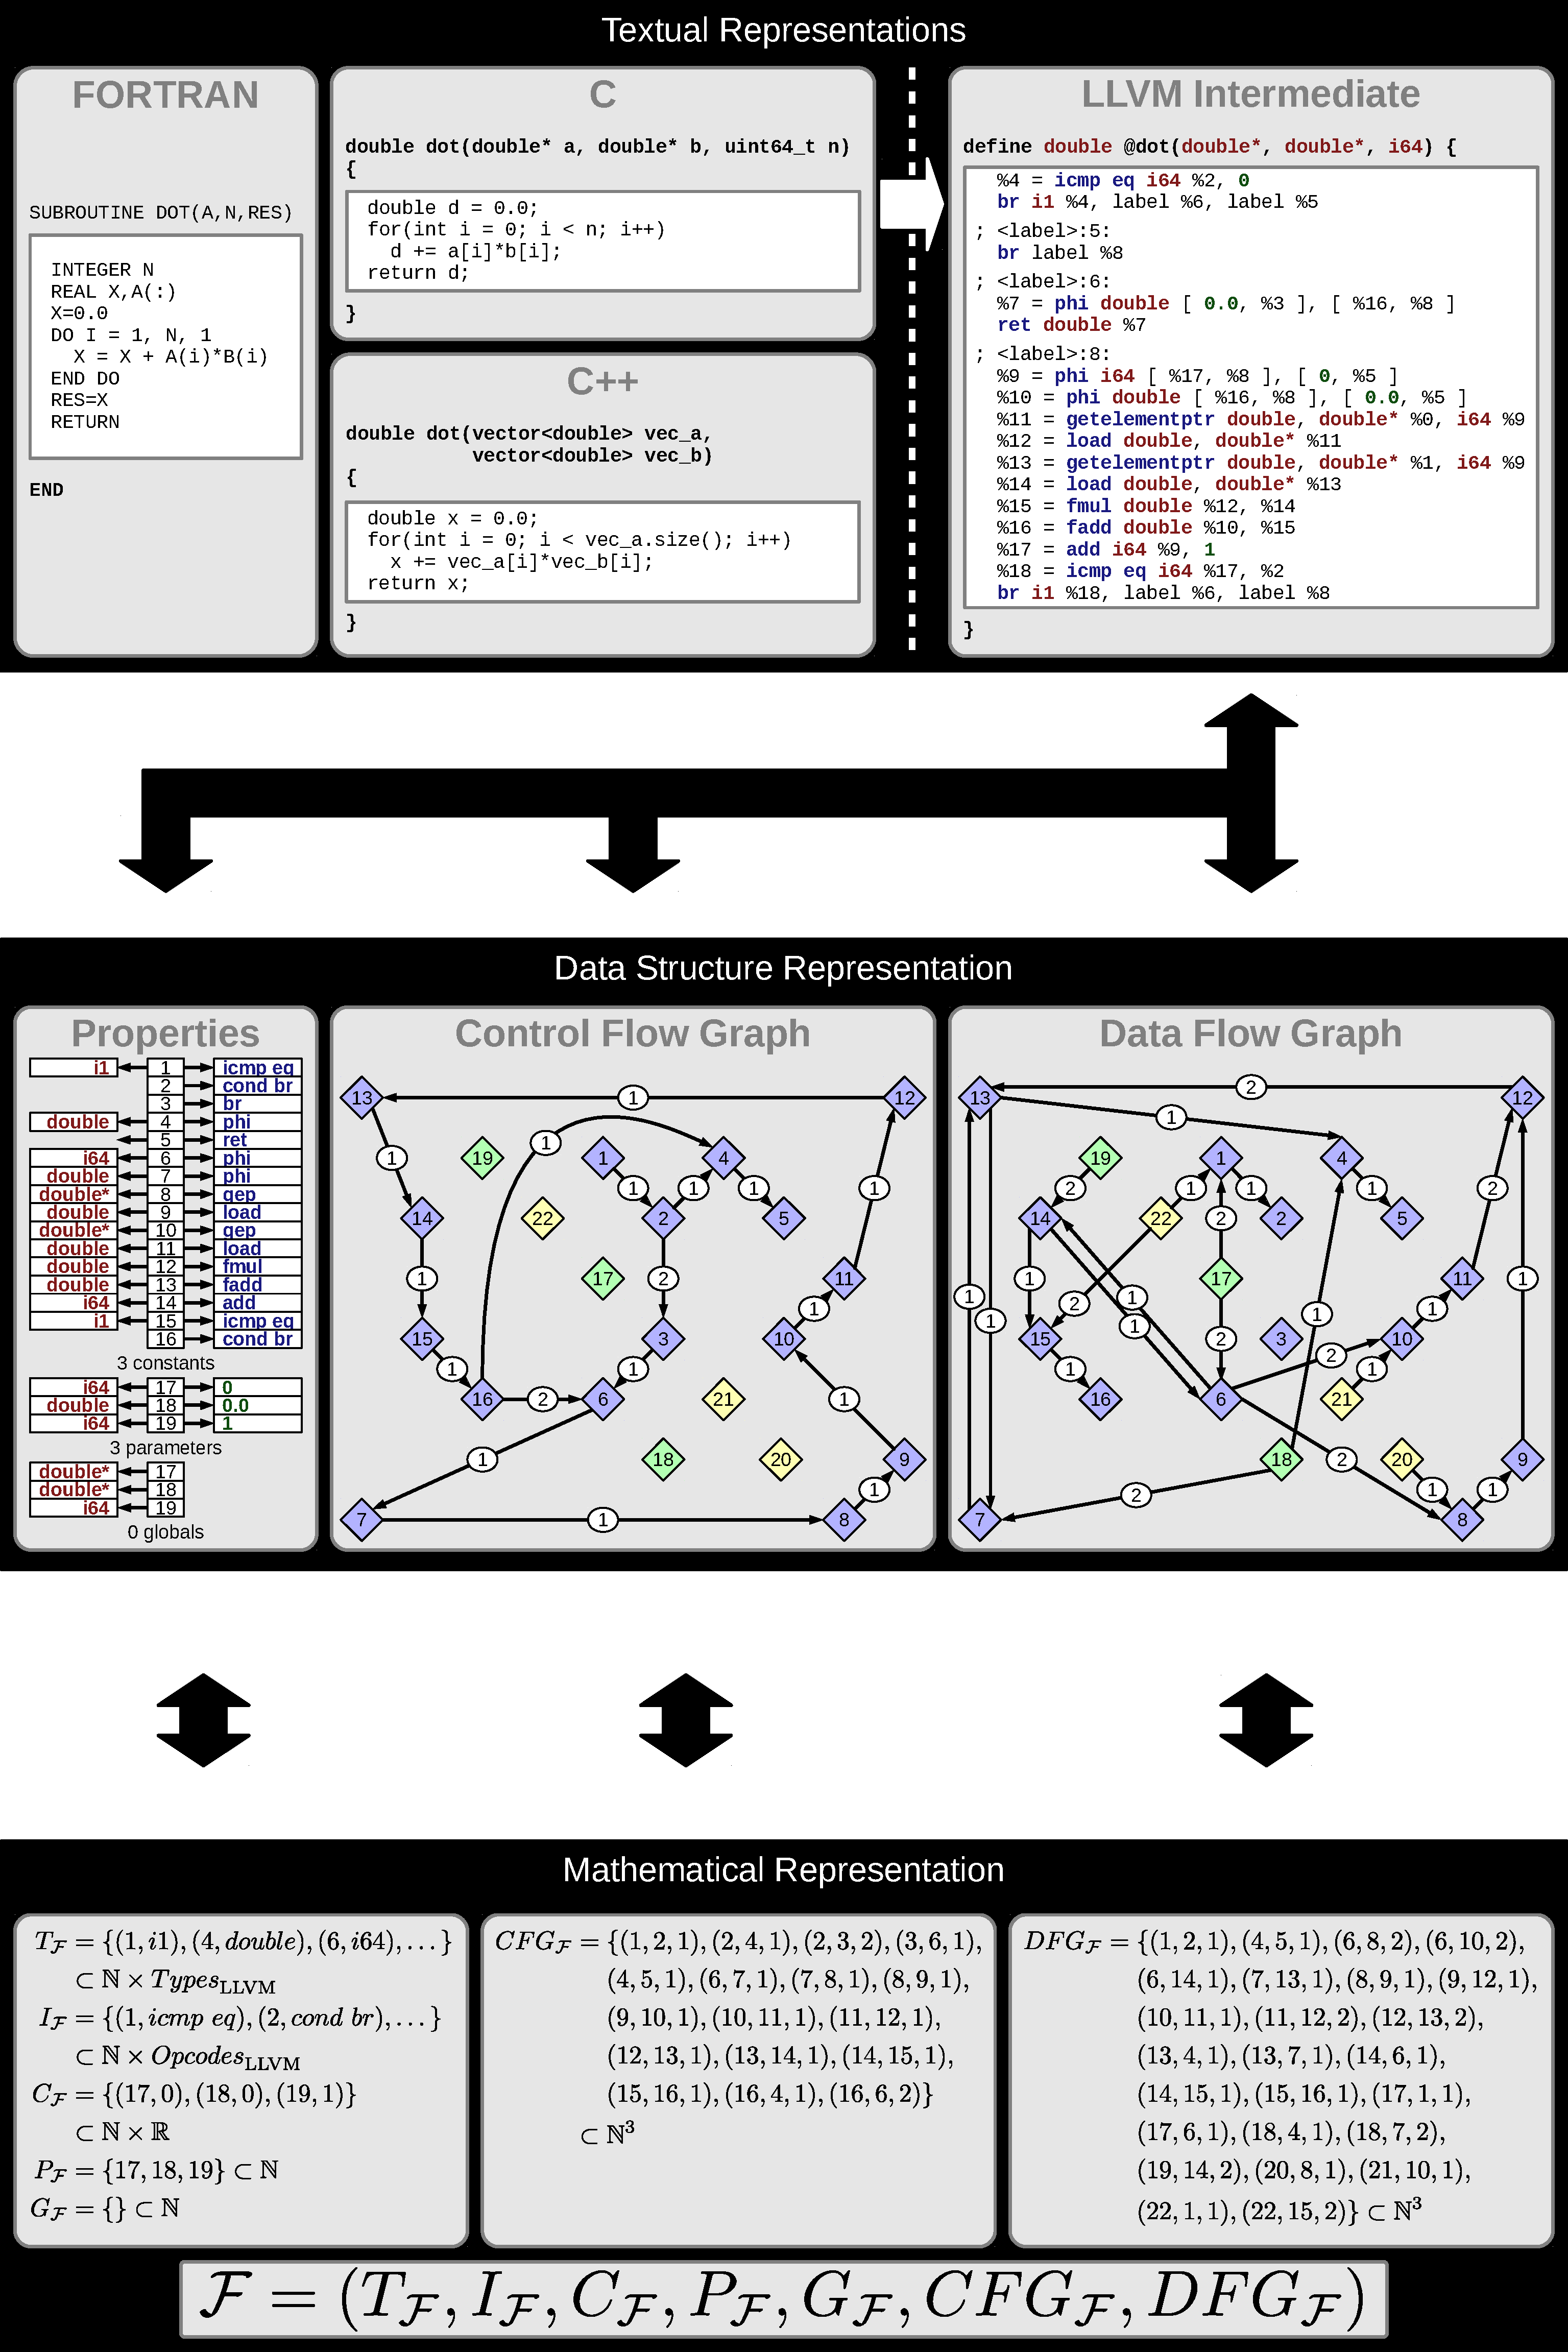
\includegraphics[width=\textwidth,height=1.5\textwidth]{figures/ssamathmodel.pdf}

\vspace{9.31595pt}
\caption{Compiler-generated SSA code is first decomposed into data flow, control
         flow and per-value attributes.
         Mathematical representations of the data are then introduced with
         notation.}
\label{fig:derivemaths}
\end{figure}

    This section derives a mathematical model of programs in single static
    assignemnt form.
    Using this model as a sound basis and mathematical notation, common compiler
    analysis problems are then reformulated.
    Later chapters will use this to define computational idioms formally, and to
    implement automatic compiler tools.
    It is not the aim here to introduce a formal operational semantics, or more
    generally to derive a model for the execution of SSA programs.
    Instead, the section will investigate the static structure, focusing on
    clear notation of the commonalities of existing SSA intermediate
    representations.

    The previous section showed how programs in SSA representations can be
    disected into several components, including control flow, data flow and
    instruction specifications.
    \autoref{fig:derivemaths} shows how this can be taken further in order to
    extract a more mathematical approach.
    At the top of the figure, different textual representations of a simple
    vector dot product are shown.
    The version of the top right is in an SSA intermediate representation: LLVM
    IR as generated by the clang compiler.

    In the middle column of \autoref{fig:derivemaths}, the information
    contained in the SSA representation is split into three components:
    Firstly, the we need a set of per-instruction properties, such as
    instruction opcodes, types and the values of constants that are used.
    Secondly, we capture the control flow graph.
    Thirdly, we capture the detailed data flow graph of the program.
    This data structure contains information about how the results of previous
    instructions are used as arguments to successive instructions.
    As we discussed in the previous section, the SSA property ensures that this
    is enough information to make the concrete register usage implicit.

    We can see this \autoref{fig:derivemaths}.
    The single static assignment property implies that it is statically knows
    at each point, which instruction produced the value in each register.
    Therefore, we can immediately identify registers with their producting
    instruction.
    Therefore we can entirely capture the interaction between instructions in
    two graphs: the control flow graph and the data flow graph.
    This is shown in in middle section of the figure.
    The data flow graph entirely replaces the concept of registers and instead
    models directly how the results from instructions are used as arguments
    in succeeding instructions.
    The control flow graph models the possible paths through the program.

    Note that we entirely removed the concepts of basic blocks and registers
    here.
    However, both can be recovered easily from the graph representations and
    hence we lost no information going from the textual representation towards
    the graph representations.

    Finally, we can model this entirely mathematical.
    We can see at the bottom of the figure, how we can model the entire function
    body as a tuple
    \begin{align*}
        \mathcal{F}=(T_\mathcal{F},I_\mathcal{F},C_\mathcal{F},P_\mathcal{F},G_\mathcal{F},CDG_\mathcal{F},DFG_\mathcal{F})\text{.}
    \end{align*}

    Note that the same model can be used abstractly for other single static
    assignment forms, only the type and opcode information as encoded via
    $Types_\text{LLVM}$ and $Opcodes_\text{LLVM}$ are specific to LLVM and need
    to be replaced.

\newpage

\subsection{Important Graph Properties}

    With our established notation, we can now transfer standard compiler
    analysis problems into this more formal language.
    Most of these are based on graph theoretic considerations, so we
    will firstly need to recapitulate some graph theory basics.
    Firstly, there is the notion of {\em cuts} of graphs, that we will introduce
    here in a hybrid version of edge based and vertex based modelling.

    \begin{definition}{Connections and Cuts}{def:cuts}
        Consider an adjacency set $E\subset\mathbb{N}\times\mathbb{N}$ of a
        directed graph and let $a,b\in\mathbb{N}$.
        \newline
        A {\em connection} between $a$ and $b$ in $E$ is a subset
        $A\subset\mathbb{N}$ such that a finite sequence $c_1,\dots,c_n$
        exists with
        \begin{gather*}
            a=c_1\hspace{1cm}c_2,\dots,c_{n-1}\in A\hspace{1cm}b=c_n\\
            (c_k,c_{k+1})\in E\hspace{1em}\text{for all}\hspace{1em}k=1,\dots,n-1.
        \end{gather*}
        A {\em cut} between $a$ and $b$ in $E$ is a subset $B\subset E$
        such that no {\em connection} between $a$ and $b$ in $E\setminus B$
        exists.
        We define the {\em set of cuts} between $a$ and $b$ in $E$ as
        \begin{align*}
            \text{Cuts}_E(a,b):=\{B\subset E\mid B\text{ is {\em cut} between $a$ and $b$ in $E$}\}
        \end{align*}
    \end{definition}

    These notions are quite intuitive, two vertices in a graph have a connection
    if one can reach the other via the available edges and by ``cutting'' these
    edges, they are no longer connected.

    These definitions are very useful in order to identify crucial properties of
    data and control flow graphs.
    Most standard is the the definition of a dominator in the control flow
    graph: An instruction $d$ is said to dominate another instruction $n$ if
    every path from the entry node to $n$ through the control flow graph must
    go through $d$.
    In our model this is of course equivalent to the following:

    \begin{definition}{Dominator}{def:dominator}
        Consider an instruction $n$ in a function $\mathcal F$.
        A {\em dominator} of $n$ in $\mathcal{F}$ is an instruction $d$ such
        that $\{(d,m)\mid(d,m)\in CFG_\mathcal{F}^*\}$ is a {\em cut} between $1$ and $n$ in $CFG_\mathcal{F}^*$.
    \end{definition}

    Another important definition is the concept of control dependence.
    Control dependence models the behaviour of conditional control flow.
    Instructions that are executed only in some control flow paths are control
    dependent on the conditional branches that preceed them.

    UNDERFUL VBOX.

    UNDERFUL VBOX.

    UNDERFUL VBOX.

    UNDERFUL VBOX.

    \begin{definition}{Control Dependence}{cdg}
        Consider instructions $a,b$.
        We say that an $b$ is control dependent on $a$ if a instructions
        $c,c'$ exist such that $(a,c),(a,c')\in CFG_\mathcal{F}^*$ and
        \begin{align*}
            \{(a,c)\}\in{}&{}\text{Cuts}_E(a,b)\\
            \{(a,c')\}\notin{}&{}\text{Cuts}_E(a,b)\text{.}
        \end{align*}
        We define the {\em control dependence graph} as follows
        \begin{align*}
            CDG_\mathcal{F}:=\{(a,b)\in\mathbb{N}^2\mid b\text{ control dependent on }a\}
        \end{align*}
    \end{definition}

\begin{figure}[p]
    \centering
    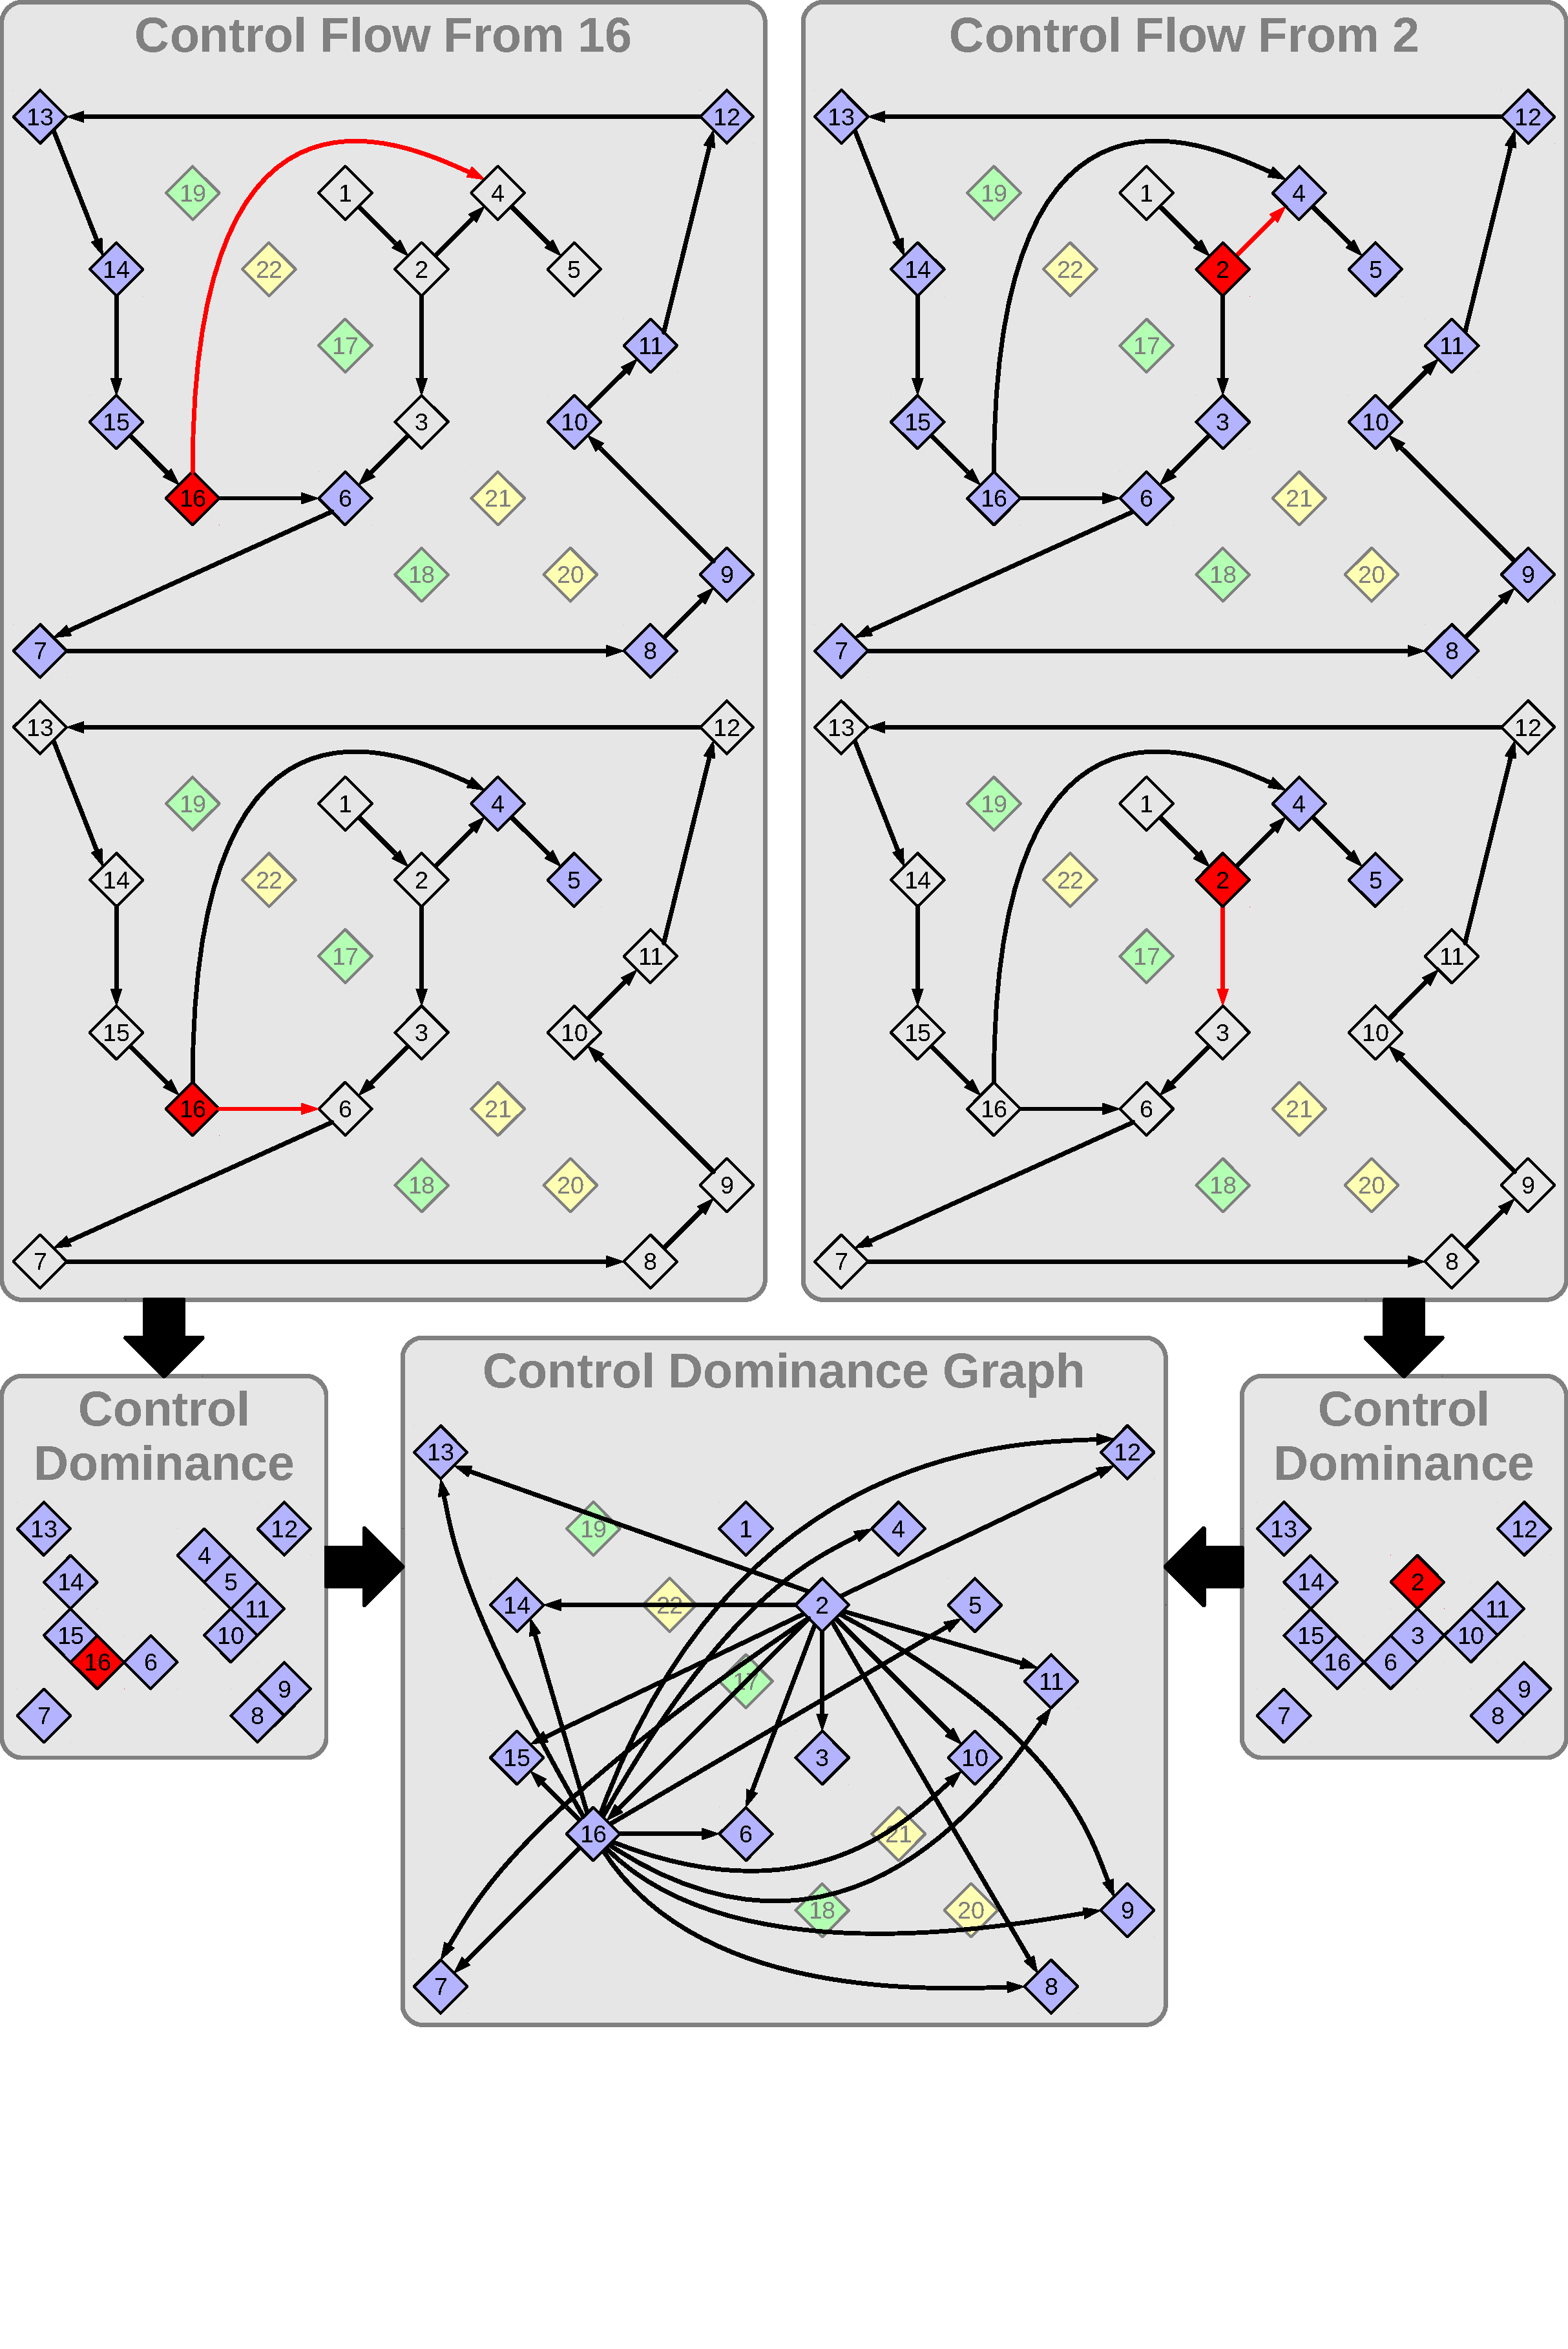
\includegraphics[width=\textwidth,height=1.5\textwidth]{figures/schaubild2.pdf}

    \vspace{27.38136pt}
    \caption{Computation of the control dependence graph.}
    \label{fig:pdg}
\end{figure}


\subsection{Control Dependence Example}

    The control dependence graph is a function of the control flow graph, as is
    directly apparent from \autoref{def:cdg}.
    We can see how an example control dependence graph is computed in
    \autoref{fig:pdg}, from the control flow graph of the \texttt{dot} function
    in \autoref{fig:derivemaths}.
    From the definition it is immediately obvious that we need to only consider
    conditional branches as origins of control dependence.

    We can consider the two conditional branches $2$ and $16$ independently.
    On the right, we consider only $2$.
    We check the defining property: On the top of the figure, all the
    instructions that are not reachable from $2$ without the edge $(2,4)$ are in
    grey.
    Below this, all instructions not reachable from $2$ without $(2,3)$ are
    grey.
    We see that $4,5$ are always reachable and $1$ is never reachable, these are
    therefore not control dependent on $2$.
    All the other instructions are control dependent on $2$.

    Once we have computed this for all conditional branches, we take the union
    on graphs and get the complete control dependence graph of the function.
    Note what this graph represents:
    Once the loop in the function has been unrolled, it contains a conditional
    and a loop.
    Eveything within the body of the conditional is control dependent on $2$.
    Everythig within the loop as well as everything afterwards is control
    dependent on $16$.


    UNDERFUL VBOX.

    UNDERFUL VBOX.

    UNDERFUL VBOX.


\subsection{Phi Dependence Graph}

    Phi nodes are fundamental in single static assignment form and need special
    care.
    The value that a phi node takes depends on from where a phi node was
    reached.
    We need to encapsulate this in a graph.

    \begin{definition}{Phi Dependence Graph}{def:pog}
        Let $p$ a phi node and $c$ a conditional branch instruction.
        We say that the outcome of $p$ depends on $c$ if there is a branch
        instruction $b$ that reaches $p$ such that $b$ is control dependent on
        $c$.

        This defines the {\em phi dependence graph} $\Phi DG_\mathcal{F}$.
    \end{definition}

\subsection{Program Dependence Graph}

    After the control flow, data flow and control dependence graph, we lastly
    introduce the {\em program dependence graph}.
    It is the most exhaustive tool that we have to describe how values depend on
    each other.

    \begin{definition}{Program Dependence Graph}{def:pdg}
        The {\em program dependence graph} is defined as the union of data flow
        and control dependence graphs.
        \begin{align*}
            PDG_\mathcal{F}:=DFG_\mathcal{F}^*\cup CDG_\mathcal{F}^*\cup\Phi DG_\mathcal{F}\text{.}
        \end{align*}
    \end{definition}

    With the program dependence graph, we can now define subsections of the
    program that are self-contained and can be separated into their own
    function.
    This works even if they contain complicated control flow.
    Firstly, we need a definition of an interface.

    \begin{definition}{Interface}{def:interface}
        Let $a\in CFG_\mathcal{F}^*$ and $b_1,\dots,b_n\in DFG_\mathcal{F}^*$.
        Furthermore let $A\subset\mathbb{N}$ a set of instructions.

        We say that $(b_1,\dots,b_n)$ is an interface to $A$ if it is a cut
        between $o$ and $A$ in $PDG_\mathcal{F}$ for any of the following $o$:
        \begin{itemize}
            \item $o$ is a paramter
            \item $o$ is impure
        \end{itemize}
    \end{definition}


\newpage
\subsection{Interface Example}

    We will now consider a non-trivial example.
    Consider this snppet of C code, implementing a function that performs a
    simple square root approximation on each element in an array of double
    precision floating point values.

\begin{figure}[ht]
\begin{lstlisting}[language=C]
void map_sqrt(size_t length, double* array)
{
    for(int i = 0; i < length; i++)
    {
        double root = 1.0;
        for(int i = 0; i < 10; i++)
            root = 0.5*(root+array[i]/root);

        array[i] = root;
    }
}
\end{lstlisting}
\caption{{\bf map$\circ$sqrt}: Apply an appriximate sqare root function to each
         element in a vector.}
\end{figure}

    Coneptually, we should be able to disentangle the square root function from
    the control flow of the outer loop.
    This is possible with the preceeding definition of {\em interfaces}.


\newpage
In single static assignment form, this code looks as follows:

\begin{lstlisting}[language=LLVM]
define void @map_sqrt(i64, double*) {
  %3 = icmp eq i64 %0, 0
  br i1 %3, label %5, label %4

; <label>:4:
  br label %6

; <label>:5:
  ret void

; <label>:6:
  %7 = phi i64 [ %10, %8 ], [ 0, %4 ]
  br label %12

; <label>:8:
  %9 = getelementptr double, double* %1, i64 %7
  store double %19, double* %9
  %10 = add nuw i64 %7, 1
  %11 = icmp eq i64 %10, %0
  br i1 %11, label %5, label %6

; <label>:12:
  %13 = phi i64 [ 0, %6 ], [ %20, %12 ]
  %14 = phi double [ 1.0, %6 ], [ %19, %12 ]
  %15 = getelementptr inbounds double, double* %1, i64 %13
  %16 = load double, double* %15
  %17 = fdiv double %16, %14
  %18 = fadd double %14, %17
  %19 = fmul double %18, 5.0
  %20 = add nuw nsw i64 %13, 1
  %21 = icmp eq i64 %20, 10
  br i1 %21, label %8, label %12
}
\end{lstlisting}

    In this example, the set $\{\%9\}$ is an interface to $\{(\%19,\%store)\}$.

\section{Formulating Constraint Problems}

    We now use these mathematical background deliberations to derive
    constraint programming on top of LLVM code.

    UNDERFUL VBOX.

    UNDERFUL VBOX.

    UNDERFUL VBOX.

    Consider the following definitions of simple binary predicates:

    \begin{align*}
     is\_branch\_inst(\mathcal F, n):= (n,\text{\bf br})\in T_\mathcal{F}\\
     is\_control\_edge(\mathcal F, n, m):= (n,m)\in CFG_\mathcal{F}^*\\
     is\_control\_dom(\mathcal F, n, m):= \\
    \end{align*}

    We can then use these predicates to define more complex constructs, such as
    single entry, single exit (SESE) regions.

    \begin{definition}{}{}{}
        A single entry single exit region is a tuple $a,b,c,d\in\mathcal N$ such
        that the following properties hold:
        \begin{align*}
            is\_control\_edge(\mathcal{F},a,b)\\
            is\_control\_edge(\mathcal{F},c,d)\\
            is\_control\_dom(\mathcal{F},c,d)\\
            is\_control\_postdom(\mathcal{F},d,c)\\
        \end{align*}
    \end{definition}